\chapter{Discussion}
\section{Design Validation}

\subsection{Robotic Testing Rig}

The testing rig, when properly lubricated to reduce mechanical impedance, performed well. The design choice to use a linear guide, instead of steel rods and ball bearings, paid off in the end - both a reduction in weight and complexity were achieved. The rig had a limited height for jump experimentation - due to the limitation in peak motor current which effectively limited the jump height to just under $0.4\ m$ the rig height was adequate. 

The testing rig enabled a number of experiments to be performed successfully including both static and dynamic tests.

\subsection{Embedded System \& GUI Design}

The embedded system design proved to be the majority of the work involved in the project. The choice of using a real time operating system to implement the communication and control enabled a complex, yes structured and easily adaptable system. The framework designed can definitely serve as a reference for future robotic projects where similar tasks are involved. 

By choosing a functional GUI, qSerialTerm, as a starting point, extensive GUI development was made possible in the short duration available. The control and command plug-ins developed, based on the same packet packing method developed during the embedded system design, are intuitive and adaptable. As further experiments were performed, Qt GUI components could be appended and integrated quickly. The cross compilation of the GUI possible for both Windows and Linux means the platform can be used for future research without concern for compatibility.

The embedded system was theoretically capable of sample rates up to approximately $800\ Hz$ with the packet sizes involved, due to limitation of the motor drivers this was not possible. The sampling rate is especially critical for virtual model applications where the response of the system needs to be consistently controlled to achieve a high fidelity response.

\section{Results Validation}

The process of modelling, simulation, implementation, and testing produced theoretical, simulated, and practical results. Using critical analysis and comparison we can validate these results. 

\subsection{Motor Current Predications}
The active compliance motor current simulation in \cref{fig:motor-current-requirements} was used to validate the motor driver peak current specification. 

The control simulation plots in \cref{fig:Control system simulation plots} showed slightly lower peak current predictions - this was expected as the control simulation was less comprehensive, whereas the active compliance motor current simulation covered all theoretical kinematic set-points. 

In reality during experimentation, as seen in \cref{fig:jump-motor-current-feedback}, the current saturated during launch, but during the other phases of jumping the current requirements predicated were correct. This was expected as the current predictions did not take into account the impulsive force needed for launching.

\Cref{fig:Current control tracking} shows the motor driver and current controller, both on-board the motor drivers and with the communication to the embedded system performed well. The minimum possible latency between current feedback and current command was achieved given the limitation of the motor driver communication system.

\subsection{Motor Torque Predications}

Motor torque predictions were performed in \cref{sec:Motor Torque Predictions}. They showed a maximum torque of approximately $4-10\ Nm$ per motor depending on the virtual model topology used. When the arc-length rotational measure was used a maximum torque of $4\ Nm$ was predicted. In practise, during the jump tests, a maximum motor torque of $4.4\ Nm$ was seen. This is not considering the motor current and torque saturation needed for launching. This validates the torque predictions simulated before testing was performed. 

\subsection{Virtual Model Fidelity}

The leg was modelled as a spring-damper system. In \cref{sec:Virtual Spring-damper Tests} this virtual model was tested to determine, amongst other aims, the fidelity of the virtual model control system. 

Various topologies were tested, and the results summarized in the analysis that followed. Although the tests showed that the natural frequency of the various responses were accurate when compared to theory, the damping factor was not easily measured for comparison - this was partially due to the use of a backwards difference velocity estimation method prior to changing to a Jacobian mapping for all further tests.

\subsection{Force Control Fidelity}

As performed in \cref{sec:Consecutive Jump Repeatability}, the experiment found that during repeated jumping, the force control system was both robust to disturbances and implemented reliable and repeatable force control.

The experiment performed in \cref{sec:Force Control Calibration and Fidelity} added to the validation of force control fidelity by showing the mechanical transparency between the motor torque and foot force coupling. In theory a linear force relationship was expected using a spring-damper model and the linear motor torque current relationship, with a varying radial offset - this was confirmed during experimentation.

Both of the above experiments show the fidelity of the force control. Although a Simulink force control simulation was performed, it was not directly comparable to the experiments, despite proving useful in determining the reliability of operation of the control system.

\section{Performance Validation}

Performance validation aims to both validate the performance of the system as originally expected during the research investigation stage, and as compared to other similar legged robots.

By considering the original problems to be investigated the following discussion can be had about the overall performance of the system:

\subsection{Problems to be Investigated}
\begin{itemize}
\item \textbf{High speed embedded system communication and packet processing:} Using a RTOS and DMA framework, high speed communication up to $800\ Hz$ was reliably achieved on the embedded system. Due to motor driver constraints this was limited to $200\ Hz$.
\item \textbf{Virtual model control for accurate end effector force output:} Virtual model control force fidelity was shown by comparing simulation and testing to theory. It was found to be accurate for the majority of the testing, but without a proper load cell system it is difficult to properly measure performance.
\item \textbf{Effective high speed kinematic control:} The kinematic control was most effectively tested during the trajectory tracking tests in \cref{sec:Trajectory Tracking}. Although accurate trajectory tracking was achieved, the high speed capabilities of the system were not extensively tested. During jump tests the maximum speed of $3\ m/s$ was tested and kinematic performance was adequate for that case.
\item \textbf{Effective use of motor drivers to achieve rapid accelerations with a direct drive BLDC motor:} The motor drivers were limited in both current peak and communication speed specifications. They performed adequately for the jump tests, but during more rapid three dimensional tests with more robotic mass or jump height needed, better motor drivers would be required.
\item \textbf{Development of a platform suitable for further use in dynamic legged motion research:} The software design is highly adaptable and capable of performing further research. The hardware design is adequate for the single vertical axis tests performed in this study, but would need to be more robust for further extensive testing.
\end{itemize}

\subsection{State of the Art Comparison}

\Cref{tbl:Robot performance comparison} provides a performance comparison of various legged robots, as compiled by \cite{Kalouche2016}.

A few of the robots that specifically use the same linkage leg design as Baleka will be compared in more depth. Although the kinematic equations derived in \cite{Duperret} were adapted for Baleka, the study did not include the necessary detail needed to compare it's performance. The GOAT leg \cite{Kalouche2016}, the ATRIAS robot \cite{jgrimes2013}, and the Minitaur robot \cite{Kenneally2016} will be critically compared.

The robots mentioned are all of different size and configurations. The GOAT leg was tested in the single leg case and the ATRIAS robot was a fully sized $60\ kg$ beast. A fair comparison between these robots would be to use the energy to mass ratio in $[J/kg]$. This ensures the energy delivered is normalized, and that the large robots don't have an unfair advantage with larger actuators.

Baleka weighed in at an energy to mass ratio of $3.9\ J/kg$, ATRIAS at $1.1\ J/kg$, GOAT at $8.0\ J/kg$, and Minitaur at $4.7\ J/kg$. The places GOAT ahead of the pack with Minitaur and Baleka following just behind. 

If on the other hand you consider the actuator mass ratio, it tells a different story. Baleka weighs in at $8.7\ J/kg$, ATRIAS at $10\ J/kg$, Minitaur at $11.75\ J/kg$, and GOAT at $16.7\ J/kg$. This means that the GOAT robot managed to get the most efficient use out of its motors, or the most energy delivered per kg of actuator. This performance measure also shows how Baleka failed to deliver as much energy due to the limitation of the motor drivers, as both the GOAT leg and Baleka leg used the same motors and virtual model control.

Considering the constraints on Baleka, it performed well for its class, delivering a middle of the range $3.9\ J/kg$. A number of the other robotic platforms did not meet these specifications, but it should also be considered that Baleka was specifically built for jumping whereas some of the robots could perform complex manoeuvres. 

Considering that Baleka was built for jumping, we should compare jump heights. Baleka achieved a maximum height of $0.4\ m$, ATRIAS $0.11\ m$, Minitaur $0.48\ m$ and GOAT $0.82\ m$. These tests are a bit more difficult to compare given the different leg topologies used. Baleka was certainly capable of performing a much higher jump given more current, but considering that the GOAT leg jumped $0.82\ m$ with approximately the same current shows that the leg design and efficiency were superior to that of Baleka, and given more time and resources should be strived for.

\begin{figure}
\centering
\subfloat[][ATRIAS.]{
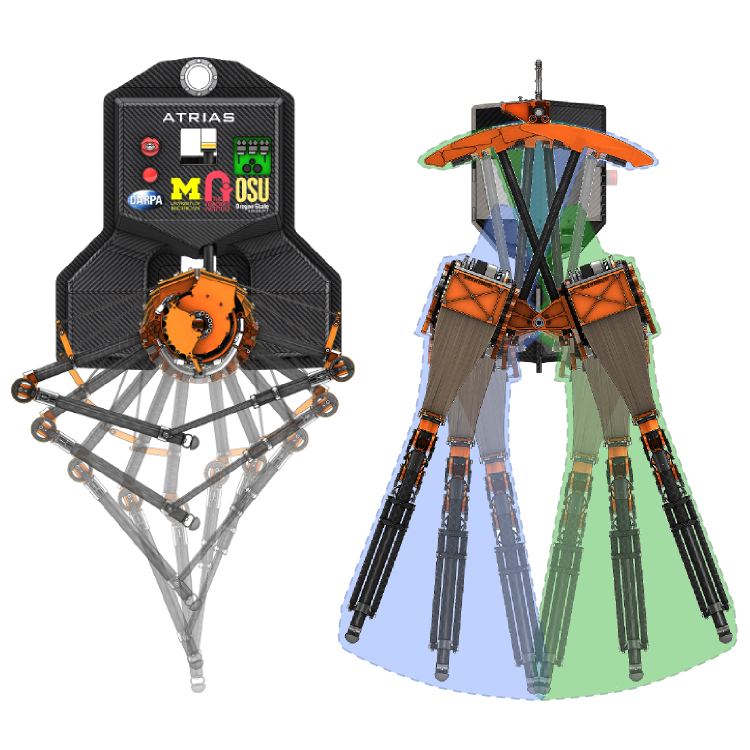
\includegraphics[width=0.3\textwidth]{images/discussion/ATRIAS.png} 
\label{fig:ATRIAS}
}
~
\subfloat[][Minitaur.]{
\includegraphics[width=0.3\textwidth]{images/discussion/Minitaur.jpeg} 
\label{fig:Minitaur}
}

\subfloat[][GOAT.]{
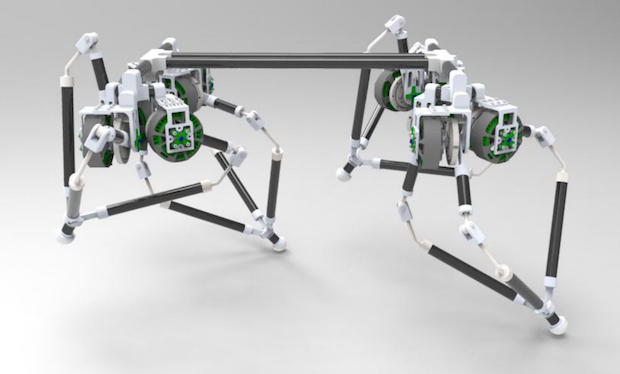
\includegraphics[width=0.3\textwidth]{images/discussion/GOAT.jpeg} 
\label{fig:GOAT}
}
\caption{Robots for performance comparison.}
\label{fig:Robots for performance comparison}
\end{figure}

\begin{table}[]
\centering
\begin{tabular}{lllllllll}
\textbf{Robot} & \textbf{\pbox{20cm}{Legs\\{[}no.{]}}} & \textbf{DoF} & \textbf{\pbox{20cm}{Leg\\Length\\{[}m{]}}} & \textbf{\pbox{20cm}{Mass\\{[}kg{]}}} & \textbf{\pbox{20cm}{Motor\\Mass\\{[}\%{]}}} & \textbf{\pbox{20cm}{Gear\\Ratio}} & \textbf{\pbox{20cm}{Jump\\Height\\{[}m{]}}} & \textbf{\pbox{20cm}{Energy\\Delivered\\{[}J{]}}} \\
\rowcolor[HTML]{67FD9A} 
Baleka         & 1                       & 2            & 0.3                         & 2.2                    & 45                           & n/a                 & 0.4                          & 8.63                              \\
Goat           & 1                       & 3            & 0.26                        & 2.5                    & 48                           & n/a                 & 0.82                         & 20.11                             \\
MIT Cheetah    & 4                       & 3            & 0.275                       & 33                     & 24                           & 5.8                 & 0.5                          & 161.9                             \\
Minitaur       & 4                       & 2            & 0.2                         & 2                      & 40                           & n/a                 & 0.48                         & 9.41                              \\
XRL            & 6                       & 1            & 0.2                         & 8                      & 11                           & 23                  & 0.425                        & 33.3                              \\
Delta Hopper   & 1                       & 3            & 0.2                         & 2                      & 38                           & n/a                 & 0.35                         & 6.9                               \\
StarlETH       & 4                       & 3            & 0.2                         & 23                     & 16                           & 100                 & 0.32                         & 72.2                              \\
HRP3La-JSK     & 2                       & 6            & 0.6                         & 54                     & 9.2                          & ??                  & 0.27                         & 143                               \\
ATRIAS         & 2                       & 3            & 0.42                        & 60                     & 11                           & 50                  & 0.11                         & 64.7                             
\end{tabular}
\caption{Legged robot performance comparison.\cite{Kalouche2016}}
\label{tbl:Robot performance comparison}
\end{table}